\documentclass[english,man]{apa6}

\usepackage{amssymb,amsmath}
\usepackage{ifxetex,ifluatex}
\usepackage{fixltx2e} % provides \textsubscript
\ifnum 0\ifxetex 1\fi\ifluatex 1\fi=0 % if pdftex
  \usepackage[T1]{fontenc}
  \usepackage[utf8]{inputenc}
\else % if luatex or xelatex
  \ifxetex
    \usepackage{mathspec}
    \usepackage{xltxtra,xunicode}
  \else
    \usepackage{fontspec}
  \fi
  \defaultfontfeatures{Mapping=tex-text,Scale=MatchLowercase}
  \newcommand{\euro}{€}
\fi
% use upquote if available, for straight quotes in verbatim environments
\IfFileExists{upquote.sty}{\usepackage{upquote}}{}
% use microtype if available
\IfFileExists{microtype.sty}{\usepackage{microtype}}{}

% Table formatting
\usepackage{longtable, booktabs}
\usepackage{lscape}
% \usepackage[counterclockwise]{rotating}   % Landscape page setup for large tables
\usepackage{multirow}		% Table styling
\usepackage{tabularx}		% Control Column width
\usepackage[flushleft]{threeparttable}	% Allows for three part tables with a specified notes section
\usepackage{threeparttablex}            % Lets threeparttable work with longtable

% Create new environments so endfloat can handle them
% \newenvironment{ltable}
%   {\begin{landscape}\begin{center}\begin{threeparttable}}
%   {\end{threeparttable}\end{center}\end{landscape}}

\newenvironment{lltable}
  {\begin{landscape}\begin{center}\begin{ThreePartTable}}
  {\end{ThreePartTable}\end{center}\end{landscape}}

  \usepackage{ifthen} % Only add declarations when endfloat package is loaded
  \ifthenelse{\equal{\string man}{\string man}}{%
   \DeclareDelayedFloatFlavor{ThreePartTable}{table} % Make endfloat play with longtable
   % \DeclareDelayedFloatFlavor{ltable}{table} % Make endfloat play with lscape
   \DeclareDelayedFloatFlavor{lltable}{table} % Make endfloat play with lscape & longtable
  }{}%



% The following enables adjusting longtable caption width to table width
% Solution found at http://golatex.de/longtable-mit-caption-so-breit-wie-die-tabelle-t15767.html
\makeatletter
\newcommand\LastLTentrywidth{1em}
\newlength\longtablewidth
\setlength{\longtablewidth}{1in}
\newcommand\getlongtablewidth{%
 \begingroup
  \ifcsname LT@\roman{LT@tables}\endcsname
  \global\longtablewidth=0pt
  \renewcommand\LT@entry[2]{\global\advance\longtablewidth by ##2\relax\gdef\LastLTentrywidth{##2}}%
  \@nameuse{LT@\roman{LT@tables}}%
  \fi
\endgroup}


  \usepackage{graphicx}
  \makeatletter
  \def\maxwidth{\ifdim\Gin@nat@width>\linewidth\linewidth\else\Gin@nat@width\fi}
  \def\maxheight{\ifdim\Gin@nat@height>\textheight\textheight\else\Gin@nat@height\fi}
  \makeatother
  % Scale images if necessary, so that they will not overflow the page
  % margins by default, and it is still possible to overwrite the defaults
  % using explicit options in \includegraphics[width, height, ...]{}
  \setkeys{Gin}{width=\maxwidth,height=\maxheight,keepaspectratio}
\ifxetex
  \usepackage[setpagesize=false, % page size defined by xetex
              unicode=false, % unicode breaks when used with xetex
              xetex]{hyperref}
\else
  \usepackage[unicode=true]{hyperref}
\fi
\hypersetup{breaklinks=true,
            pdfauthor={},
            pdftitle={Have researchers increased reporting of outliers in response to the reproducability crisis?},
            colorlinks=true,
            citecolor=blue,
            urlcolor=blue,
            linkcolor=black,
            pdfborder={0 0 0}}
\urlstyle{same}  % don't use monospace font for urls

\setlength{\parindent}{0pt}
%\setlength{\parskip}{0pt plus 0pt minus 0pt}

\setlength{\emergencystretch}{3em}  % prevent overfull lines

\ifxetex
  \usepackage{polyglossia}
  \setmainlanguage{}
\else
  \usepackage[english]{babel}
\fi

% Manuscript styling
\captionsetup{font=singlespacing,justification=justified}
\usepackage{csquotes}
\usepackage{upgreek}

 % Line numbering
  \usepackage{lineno}
  \linenumbers


\usepackage{tikz} % Variable definition to generate author note

% fix for \tightlist problem in pandoc 1.14
\providecommand{\tightlist}{%
  \setlength{\itemsep}{0pt}\setlength{\parskip}{0pt}}

% Essential manuscript parts
  \title{Have researchers increased reporting of outliers in response to the
reproducability crisis?}

  \shorttitle{Outlier reporting}


  \author{K. D. Valentine\textsuperscript{1}, Erin M. Buchanan\textsuperscript{2}, Arielle Cunningham\textsuperscript{2}, Tabetha Hopke\textsuperscript{2}, Addie Wikowsky\textsuperscript{2}, \& Haley Wilson\textsuperscript{2}}

  % \def\affdep{{"", "", "", "", "", ""}}%
  % \def\affcity{{"", "", "", "", "", ""}}%

  \affiliation{
    \vspace{0.5cm}
          \textsuperscript{1} University of Missouri\\
          \textsuperscript{2} Missouri State University  }

  \authornote{
    K. D. Valentine is a Ph.D.~candidate at the University of Missouri. Erin
    M. Buchanan is an Associate Professor of Quantitative Psychology at
    Missouri State University. Arielle Cunningham, Tabetha Hopke, Addie
    Wikowsky, and Haley Wilson are master's candidates at Missouri State
    University.
    
    Correspondence concerning this article should be addressed to K. D.
    Valentine, 210 McAlester Hall, Columbia, MO, 65211. E-mail:
    \href{mailto:kdvdnf@mail.missouri.edu}{\nolinkurl{kdvdnf@mail.missouri.edu}}
  }


  \abstract{Psychology is currently experiencing a ``renaissance'' where replication
and reproducibility of published reports is the forefront conversation
in the field. While researchers have worked to discuss possible problems
and solutions, work has yet to uncover how this new culture may have
altered reporting practices in the social sciences. As outliers can bias
both descriptive and inferential statistics, the examination for these
data points is essential to any analysis using these parameters. We
quantified the rates of reporting of outliers within psychology at two
time points: 2012 when the replication crisis was born, and 2017, after
the publication of reports concerning replication, questionable research
practices, and transparency. A total of 2235 experiments were identified
and analyzed, finding an increase in reporting of outliers from only
15.7\% of experiments mentioning outliers in 2012 to 25.0\% in 2017. We
delved into differences across years given the psychological field or
statistical analysis that experiment employed. Further, we inspect
whether outliers mentioned are whole participant observations or data
points, and what reasons authors gave for stating the observation was
deviant. We conclude that while report rates are improving overall,
there is still room for improvement in the reporting practices of
psychological scientists which can only aid in strengthening our
science.}
  \keywords{outlier, influential observation, replication \\

    
  }





\usepackage{amsthm}
\newtheorem{theorem}{Theorem}[section]
\newtheorem{lemma}{Lemma}[section]
\theoremstyle{definition}
\newtheorem{definition}{Definition}[section]
\newtheorem{corollary}{Corollary}[section]
\newtheorem{proposition}{Proposition}[section]
\theoremstyle{definition}
\newtheorem{example}{Example}[section]
\theoremstyle{definition}
\newtheorem{exercise}{Exercise}[section]
\theoremstyle{remark}
\newtheorem*{remark}{Remark}
\newtheorem*{solution}{Solution}
\begin{document}

\maketitle

\setcounter{secnumdepth}{0}



Psychology is undergoing a \enquote{renaissance} in which focus has
shifted to the replication and reproducibility of current published
reports (Etz \& Vandekerckhove, 2016; Lindsay, 2015; Nelson, Simmons, \&
Simonsohn, 2018; Open Science Collaboration, 2015; van Elk et al.,
2015). A main concern has been the difficulty in replicating phenomena,
often attributed to publication bias (Ferguson \& Brannick, 2012), the
use and misuse of \emph{p}-values (Gigerenzer, 2004; Ioannidis, 2005),
and researcher degrees of freedom (Simmons, Nelson, \& Simonsohn, 2011).
In particular, this analysis focused on one facet of questionable
research practices (QRPs) that affect potential replication,
specifically, the selective removal or inclusion of data points.

As outlined by Nelson et al. (2018), the social sciences turned inward
to examine their practices due to the publication of unbelievable data
(Wagenmakers, Wetzels, Borsboom, \& van der Maas, 2011), academic fraud
(Simonsohn, 2013), failures to replicate important findings (Doyen,
Klein, Pichon, \& Cleeremans, 2012), and the beginning of the Open
Science Framework (Nosek, 2015). These combined forces led to the
current focus on QRPs and \emph{p}-hacking and the investigation
potential solutions to these problems. Recommendations included
integrating effect sizes into results (Cumming, 2008; Lakens, 2013),
encouraging researchers to be transparent about their research
practices, including not only the design and execution of their
experiments, but especially the data preparation and resulting analyses
(Simmons et al., 2011), attempting and interpreting well thought out
replication studies (Asendorpf et al., 2013; Maxwell, Lau, \& Howard,
2015), altering the way we think about \emph{p}-values (Benjamin et al.,
2018; Lakens et al., 2018; Valentine, Buchanan, Scofield, \& Beauchamp,
2017), and restructuring incentives (Nosek, Spies, \& Motyl, 2012).
Additionally, Klein et al. (2014) developed the Many Labs project to aid
in data collection for increased power, while the Open Science
Collaboration (2015) published their findings from a combined many labs
approach about the replication of phenomena in psychology.

While we have seen vast discussion of the problems and proposed
solutions, research has yet to determine how this new culture may have
impacted reporting practices of researchers. Herein, we aim specifically
to quantify the rates of reporting of outliers within psychology at two
time points: 2012 when the replication crisis was born (Pashler \&
Wagenmakers, 2012), and 2017, after the publication of reports
concerning QPRs, replication, and transparency (Miguel et al., 2014).

\subsection{Outliers}\label{outliers}

Bernoulli first mentioned outliers in 1777 starting the long history of
examining for discrepant observations (Bernoulli \& Allen, 1961), which
can bias both descriptive and inferential statistics (Cook \& Weisberg,
1980; Stevens, 1984; Yuan \& Bentler, 2001; Zimmerman, 1994). Therefore,
the examination for these data points is essential to any analysis using
these parameters, as outliers can impact study results. Outliers have
been defined as influential observations or fringliers but specifically
we use the definition of \enquote{an observation which being atypical
and/or erroneous deviates decidedly from the general behavior of
experimental data with respect to the criteria which is to be analyzed
on it} (Muñoz-Garcia, Moreno-Rebollo, \& Pascual-Acosta, 1990, pg 217).
However, the definition of outliers can vary from researcher to
researcher, as a wide range of graphical and statistical options are
available for outlier detection (Beckman \& Cook, 1983; Hodge \& Austin,
2004; Orr, Sackett, \& Dubois, 1991; Osborne \& Overbay, 2004). For
example, Tabachnick and Fidell (2012) outline several of the most
popular detection methods including visual data inspection, residual
statistics, a set number of standard deviations, Mahalanobis distance,
Leverage, and Cook's distances. Before the serious focus on QRPs, the
information regarding outlier detection as part of data screening was
often excluded from publication, particularly if a journal page limit
requirement needed to be considered. Consider, for example, Orr et al.
(1991), who inspected 100 Industrial/Organizational Psychology personnel
studies and found no mention of outliers.

However, outlier detection and removal is likely part of a researchers
data screening procedure, even if it does not make the research
publication. LeBel et al. (2013) that 11\% of psychology researchers
stated that they had not reported excluding participants for being
outliers in their papers. Fiedler and Schwarz (2016) suggested that more
than a quarter of researchers decide whether to exclude data only after
looking at the impact of doing so. Bakker and Wicherts (2014)
investigated the effects of outliers on published analyses, and while
they did not find that they affected the surveyed results, they do
report that these findings are likely biased by the non-reporting of
data screening procedures, as sample sizes and degrees of freedom often
did not match. These studies indicate that a lack of transparency in
data manipulation and reporting is problematic.

By keeping outliers in a dataset, analyses are more likely to have
increased error variance (depending on sample size, Orr et al., 1991),
biased estimates (Osborne \& Overbay, 2004), and reduced effect size and
power (Orr et al., 1991; Osborne \& Overbay, 2004), which can alter the
results of the analysis and lead to falsely supporting (Type I error),
or denying a claim (Type II error). Inconsistencies in the treatment and
publication of outliers could also lead to the failures to replicate
previous work, as it would be difficult to replicate analyses that have
been \emph{p}-hacked into \enquote{just-significant} results (Leggett,
Thomas, Loetscher, \& Nicholls, 2013; Nelson et al., 2018). The
influence of this practice can be wide spread, as non-reporting of data
manipulation can negatively affect meta-analyses, effect size, and
sample size estimates for study planning. On the other hand, outliers do
not always need to be seen as nuisance, as they will often be
informative to researchers as they can encourage the diagnosis, change,
and evolution of a research model (Beckman \& Cook, 1983). Taken
together, a lack of reporting of outlier practices can lead to
furthering unwarranted avenues of research, ignoring important
information, creating erroneous theories, and failure to replicate, all
of which serve to weaken the sciences. Clarifying the presence or
absence of outliers, how they were assessed, and how they were handled,
can improve our transparency and replicability, and ultimately help to
strengthen our science.

The current zeitgeist of increased transparency and reproducibility
applies not only to the manner in which data is collected, but also the
various ways the data is transformed, cleaned, pared down, and analyzed.
Therefore, it can be argued that it is just as important for a
researcher to state how they identified outliers within their data, how
the outliers were handled, and how this choice of handling impacted the
estimates and conclusions of their analyses, as it is for them to report
their sample size. Given the timing of the renaissance, we expected to
find a positive change in reporting ratings for outliers in 2017, as
compared to 2012. This report spans a wide range of psychological
sub-domains, however, we also expected the impact of the Open Science
Collaboration (2015) publication to affect social and cognitive
psychology more than other fields.

\section{Method}\label{method}

\subsection{Fields}\label{fields}

A list of psychological sub-domains was created to begin the search for
appropriate journals to include. The authors brainstormed the list of
topics (shown in Table \ref{tab:info-table}) by first listing major
research areas in psychology (i.e., cognitive, clinical, social, etc.).
Second, a list of common courses offered at large universities was
consulted to add to the list of fields. Last, the American Psychological
Association's list of divisions was examined for any potential missed
fields. The topic list was created to capture large fields of psychology
with small overlap (i.e., cognition and neuropsychology) while avoiding
specific sub-fields of topics (i.e., cognition overall versus perception
and memory only journals). Sixteen fields were initially identified,
however only thirteen were included in final analysis due to limitations
noted below.

\subsection{Journals}\label{journals}

Once these fields were agreed upon, researchers used various search
sources (Google, EBSCO host databases) to find journals that were
dedicated to each broad topic. Journals were included if they appeared
to publish a wide range of articles within the selected fields. A list
of journals, publishers, and impact factors (as noted by each journals
website in Spring of 2013 and 2018) were identified for each field. Two
journals from each field were selected based on the following criteria:
1) impact factors over one at minimum, 2) a mix of publishers, if
possible, and 3) availability due to university resources. These
journals, impact factors, and publishers are shown in the online
supplemental materials at \url{https://osf.io/52mqw/}.

\subsection{Articles}\label{articles}

Fifty articles from each journal were examined for data analysis: 25
articles were collected beginning in Spring 2013 for 2012 and in Fall
2017. Data collection of articles started at the last volume publication
from the given year (2012 or 2017) and progressed backwards until 25
articles had been found. Articles were included if they met the
following criteria: 1) included data analyses, 2) included multiple
participants or data-points, and 3) analyses were based on human
subjects or stimuli. Therefore, we excluded theory articles, animal
populations, and single subject designs. Based on review for the 2012
articles, three fields were excluded. Applied Behavior Analysis articles
predominantly included single-subject designs, evolutionary psychology
articles were primarily theory articles, and statistics related journal
articles were based on user simulated data with a specific set of
characteristics. Since none of these themes fit into our analysis of
understanding data screening with human subject samples, we excluded
those three fields from analyses.

\subsection{Data Processing}\label{data-processing}

Each article was then reviewed for key components of data analysis. Each
experiment in an article was coded separately. For each experiment, the
type of analysis conducted, number of participants/stimuli analyzed, and
whether or not they made any mention of outliers were coded.

\subsubsection{Analysis types}\label{analysis-types}

Types of analyses were broadly defined as basic statistics (descriptive
statistics, \emph{z}-scores, \emph{t}-tests, and correlations), ANOVAs,
regressions, chi-squares, non-parametric statistics, modeling, and
Bayesian/other analyses.

\subsubsection{Outlier coding}\label{outlier-coding}

For outliers, we used a dichotomous yes/no for if they were mentioned in
an article. Outliers were not limited to simple statistical analysis of
discrepant responses, but we also checked for specific exclusion
criteria that were not related to missing data or study characteristics
(i.e., we did not consider it an outlier if they were only looking for
older adults). If so, we coded information about outliers into four
types: 1) people, 2) data points, 3) both, or 4) none found. The
distinction between people and data points was if individual trials were
eliminated or if entire participant data was eliminated. We found that a
unique code for data points was important for analyses with response
time studies where individual participants were not omitted but rather
specific data trials were eliminated.

Then, for those articles that mentioned outliers, the author's decision
for how to handle the outliers was coded into whether they removed
participants/data points, left these outliers in the analysis, or
winsorized the data points. Experiments were coded for whether they
tested the analyses with, without, or both for determination of their
effect on the study. If they removed outliers, a new sample size was
recorded; although, this data was not analyzed, as we determined it was
conflated with removal of other types of data unrelated to the interest
of this paper (i.e., missing data). Lastly, we coded the reasoning for
outlier detection as one or more of the following: 1) Statistical reason
(i.e., used numbers to define odd or deviant behavior in responding,
such as \emph{z}-score or Mahalanobis distance scores), 2) Participant
error (i.e., failed attention checks, did not follow instructions, or
low quality data because of participant problems), and 3) Unusable data
(i.e., inside knowledge of the study or experimenter/technological
problems).

\section{Results}\label{results}

\subsection{Data Analytic Plan}\label{data-analytic-plan}

Because each article constituted multiple data points within the dataset
which were each nested within a particular journal, a multilevel model
(MLM) was used to control for correlated error (Gelman, 2006). Pinheiro,
Bates, Debroy, Sarkar, and Team (2017) \emph{nlme} package in \emph{R}
was used to calculate these analyses. A maximum likelihood logistic
multilevel model was used to examine how the year in which the
experiment was published predicted the likelihood of mentioning outliers
(yes/no) while including a random intercept for journal. This model was
run over all of the data, as well as broken down by sub-fields or
analyses in order to glean a more detailed account of the effect of year
on outlier reporting. Additionally, three MLMs were analyzed attempting
to individually predict each outlier reason (i.e., statistical reason
yes/no; unusable data yes/no; participant reason yes/no) given the year
while including a random intercept for journal. We futher explored
whether these outliers were people or data points, how outliers were
handled, and the reasons data were named outliers with descriptive
statistics. All code and data can be viewed inline with the manuscript,
which was written with the \emph{papaja} package (Aust \& Barth, 2017).

\subsection{Overall Outliers}\label{overall-outliers}

Data processing resulted in a total of 2235 experiments being coded,
1085 of which were from 2012 or prior, with the additional 1150 being
from 2017 or prior. Investigating reporting of outliers, we found that
in 2012, 15.7\% of experiments mentioned outliers, while in 2017 25.0\%
of experiments mentioned outliers. Actual publication year was used to
predict outlier mention (yes/no) with a random intercept for journal, as
described above. We did not use publication year as a dichotomous
variable, as not all articles were from 2012 or 2017 because of
publication rates (i.e., number of articles and issues per year) and
article exclusions. We found that publication year predicted outlier
mentions, \emph{Z} = 5.78, \emph{p} \textless{} .001. Each year,
experiments were 13.5\% more likely to report outliers as the previous
year.

\subsection{Fields}\label{fields-1}

Further exploration reveals that differences in reporting between years
arise between fields which can be seen in Table \ref{tab:info-table}.
Figure \ref{fig:type-graph} displays the percentage of outlier mentions
of each field colored by year examined. A MLM was analyzed for each
field using journal as a random intercept to determine the influence of
year of publication on outlier reporting rates. Specifically, if we look
at the change in reporting for each field analyzed at the level of the
experiment, we find the largest changes in forensic (44.9\% more likely
to report), social (33.7\%), and I/O (33.4\%), followed by developmental
(19.6\%), counseling (20.2\%), and cognitive (15.2\%). In support of our
hypothesis, we found that social and cognitive fields showed increases
in their outlier reporting; however, it was encouraging to see positive
trends in other fields as well. These analyses show that in some fields,
including our overall and neurological fields, we found a decrease in
reporting across years, although these changes were not significant.

The analyses shown below were exploratory based on the findings when
coding each experiment for outlier data. We explored the relationship of
outlier reporting to the type of analysis used to support research
hypotheses, reasons for why outliers were excluded, as well as the type
of outlier excluded from the study.

\begin{figure}
\centering
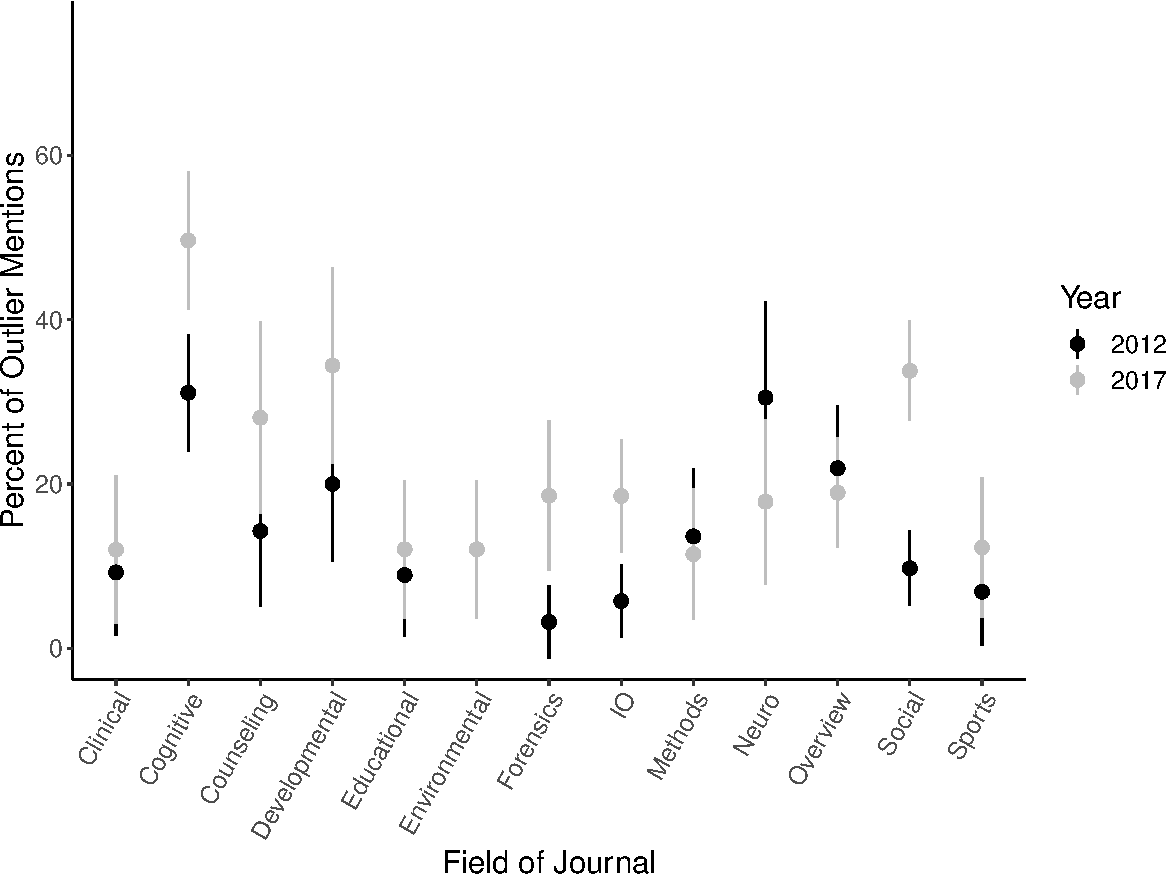
\includegraphics{outliers_manuscript_files/figure-latex/type-graph-1.pdf}
\caption{\label{fig:type-graph}Percent of outlier mentions by sub-domain
field and year examined. Error bars represent 95\% confidence interval.}
\end{figure}

\begin{table}[tbp]
\begin{center}
\begin{threeparttable}
\caption{\label{tab:info-table}Outlier Reporting by Field Across Years}
\begin{tabular}{lccccccc}
\toprule
Field & \% 12 & $N$ 12 & \% 17 & $N$ 17 & OR & $Z$ & $p$\\
\midrule
Clinical & 9.3 & 54 & 12.0 & 50 & 1.06 & 0.43 & .665\\
Cognitive & 31.1 & 164 & 49.6 & 135 & 1.15 & 3.05 & .002\\
Counseling & 14.3 & 56 & 28.1 & 57 & 1.20 & 1.91 & .056\\
Developmental & 20.0 & 70 & 34.4 & 61 & 1.20 & 2.20 & .028\\
Educational & 8.9 & 56 & 12.1 & 58 & 1.07 & 0.54 & .586\\
Environmental & 12.1 & 58 & 12.1 & 58 & 1.01 & 0.05 & .957\\
Forensics & 3.2 & 62 & 18.6 & 70 & 1.45 & 2.50 & .012\\
IO & 5.8 & 104 & 19.4 & 124 & 1.35 & 3.04 & .002\\
Methods & 13.6 & 66 & 11.7 & 60 & 1.01 & 0.08 & .933\\
Neuro & 30.5 & 59 & 17.9 & 56 & 0.87 & -1.55 & .121\\
Overview & 21.9 & 114 & 18.9 & 132 & 0.96 & -0.64 & .523\\
Social & 9.8 & 164 & 33.8 & 231 & 1.34 & 5.08 & < .001\\
Sports & 6.9 & 58 & 12.3 & 57 & 1.08 & 0.64 & .522\\
\bottomrule
\end{tabular}
\end{threeparttable}
\end{center}
\end{table}

\subsection{Analyses Type}\label{analyses-type}

\begin{figure}
\centering
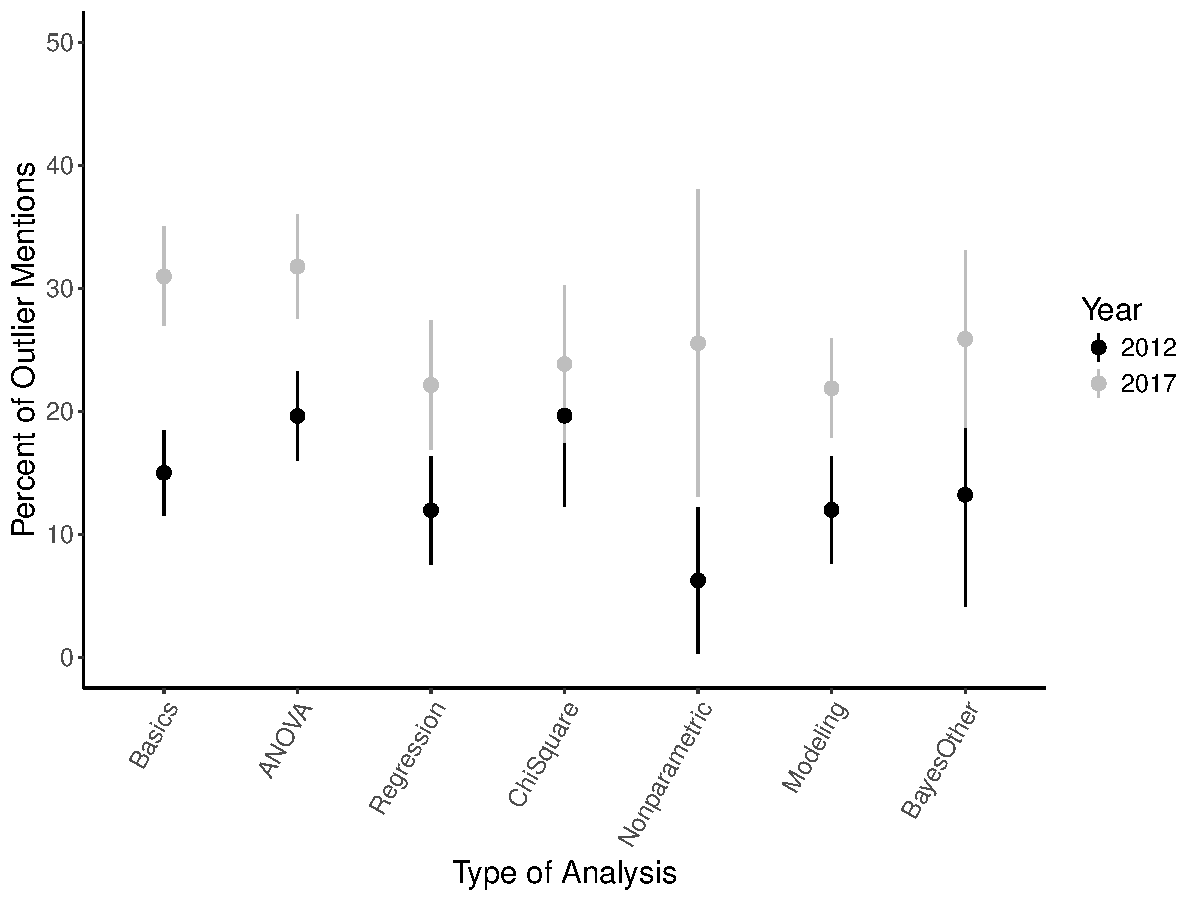
\includegraphics{outliers_manuscript_files/figure-latex/analyses-graph-1.pdf}
\caption{\label{fig:analyses-graph}Percent of outlier mentions by analysis
type and year examined. Error bars represent 95\% confidence interval.}
\end{figure}

\begin{table}[tbp]
\begin{center}
\begin{threeparttable}
\caption{\label{tab:analysis-table}Outlier Reporting by Analysis Type Across Years}
\begin{tabular}{lccccccc}
\toprule
Analysis & \% 12 & $N$ 12 & \% 17 & $N$ 17 & OR & $Z$ & $p$\\
\midrule
Basic Statistics & 15.0 & 407 & 31.0 & 507 & 1.23 & 5.86 & < .001\\
ANOVA & 19.6 & 469 & 31.8 & 466 & 1.14 & 4.40 & < .001\\
Regression & 12.0 & 209 & 22.1 & 244 & 1.15 & 2.62 & .009\\
Chi-Square & 19.6 & 112 & 23.8 & 172 & 1.04 & 0.59 & .557\\
Non-Parametric & 6.2 & 64 & 25.5 & 47 & 1.38 & 2.67 & .008\\
Modeling & 12.0 & 217 & 21.9 & 407 & 1.12 & 2.20 & .028\\
Bayesian or Other & 13.2 & 53 & 25.9 & 143 & 1.23 & 1.61 & .107\\
\bottomrule
\end{tabular}
\end{threeparttable}
\end{center}
\end{table}

Table \ref{tab:analysis-table} indicates the types of analyses across
years that mention outliers, and Figure \ref{fig:analyses-graph}
visually depicts these findings. An increase in reporting was found for
non-parametric statistics (38.2\%), basic statistics (22.6\%),
regression (15.0\%), ANOVA (14.3\%), and modeling (11.8\%). Bayesian and
other statistics additionally showed a comparable increase, 23.4\%,
which was not a significant change over years.

\subsection{Type of Outlier}\label{type-of-outlier}

In our review, the majority of outliers mentioned referred to people
(65.9\%) as opposed to data points (25.4\%), or both people and data
points (5.7\%), and a final (3.1\%) of experiments mentioned outliers
but did not specify a type, just that they found none. The trends across
years were examined for mentioning outliers (yes/no) for both people and
data points, dropping the both and none found categories due to small
size. Therefore, the dependent variable was outlier mention where the
\enquote{yes} category indicated either the people or data point
categories separately. The mentions of excluding participants increased
across years, 17.1\%, \emph{Z} = 5.99, \emph{p} \textless{} .001, while
the mention of data point exclusion was consistent across years, 4.5\%,
\emph{Z} = 1.11, \emph{p} = .268. When handling these data, some
experiments chose to winzorize the data (0.7\%), most analyzed the data
without the observations (88.6\%), some analyzed the data with the
observations (7.4\%), and some conducted analyses both with and without
the observations (3.4\%).

\subsection{Reason for Exclusion}\label{reason-for-exclusion}

We found that researchers often used multiple criterion checks for
outlier coding, as one study might exclude participants for exceeding a
standard deviation cut-off, while also excluding participants for low
effort data. Therefore, reason coding was not unique for each
experiment, and each experiment could have one to three reasons for data
exclusion. Statistical reasoning was the largest reported exclusion
criteria of papers that mentioned outliers at 58.0\%. Next, participant
reasons followed with 50.3\% of outlier mentions, and unusable data was
coded in 6.3\% of experiments that mentioned outliers. To examine the
trend over time, we used a similar MLM analysis as described in the our
data analytic plan, with journal as a random intercept, year as the
independent variable, and the mention of type of outlier (yes/no for
participant, statistical, and unusable data) as the dependent variables
separately. Statistical reasons decreased over the years by 8.4\%,
\emph{Z} = -1.91, \emph{p} = .056. Participant reasons increased over
time by 13.7\%, \emph{Z} = 2.92, \emph{p} = .004. Unusable data
increased by about 5.3\%, \emph{Z} = 0.59, \emph{p} = .554.

\section{Discussion}\label{discussion}

We hypothesized that report rates for outliers would increase overall in
experiments from 2012 to 2017, and we largely found support for this
hypothesis. We additionally hypothesized larger increases in report
rates of outliers for the domains of social and cognitive psychology
because of the overwhelming response to the Open Science Collaboration
(2015) publication. This hypothesis was supported, with increases for
both areas, along with most other sub-domains in our study. Social and
cognitive psychology publications included the most experiments in their
papers, and reporting outliers for each experiment and analysis will be
crucial for future studies or meta-analyses. While improvements in
reporting can be seen in almost all fields, it is worthwhile to note
that in 2017 the average proportion of experiments reporting outliers
was still only 25.0\%, with some fields as low as approximately 12\%.
While the effort of many fields should not be overlooked, we suggest
that there is still room for improvement overall.

All analytic techniques presented in these experiments showed increased
reporting over time, ranging from ranging from 11.8\% for modeling to
38.2\% for nonparametric statistics. Of all outliers reported, we found
that the majority discussed were people (65.9), and that while exclusion
of people as outliers increased from 2012 to 2017, exclusion of outlying
data points remained consistent across time. Most experiments cited
outliers as those found through statistical means (e.g., Mahalanobis
distance, leverage, or a standard deviation rule) and/or participant
reasons (e.g., failed attention checks or failure to follow
instructions), but a small subset were cited as unusable data (e.g.,
individuals who believed the procedure was staged or participants whose
position in a room was never recorded by the experimenter). These
findings suggest that not only is discussion of outliers important for
the study at hand, but also for future studies. Given insight into ways
data can become unusable, a researcher is better equipped to prepare for
and deter unusable data from arising in future studies through knowledge
of past failures that can improve their research design.

Given the frequentist nature of most psychological work, and the impact
those outliers can have on these statistics (Cook \& Weisberg, 1980;
Stevens, 1984), research would be well served if authors described
outlier data analyis in their reports. One confounding issue may be
journal word limits. The Open Science Framework provides the option to
publish online supplemental materials that can be referenced in
manuscripts with permanant identifiers (i.e., weblinks and dois).
Potentially, if journal or reviewer comments indicate shortening data
analyses sections, the detailed specifics of these plans can be shifted
to these online resources. While the best practice may be to include
this information in the published article, as Bakker and Wicherts (2014)
notes that sample size and degrees of freedom are often inconsistent and
difficult to follow in publications, online materials can be useful when
that option is restricted.

We implore researchers not to overlook the importance of visualizing
your data and identifying data that may not fall within the expected
range or pattern of the sample. Currently, there are online tools that
can assist even the most junior researcher in the cleaning of data,
including outlier detection and handling, for almost any type of
analysis. From online courses (e.g., Coursera.org, DataCamp.com), free
software with plugins (jamovi project, 2018; e.g., JASP and jamovi; JASP
Team, 2018), and YouTube tutorials that detail the step by step
procedures (avaliable from the second author at StatsTools.com),
inexperienced researchers can learn more for better reporting and
statistical practices. Further, we implore those who are reviewers and
editors to consider data screening procedures when assessing research
articles and request this information be added when it is absent from a
report. This article spotlights that positive changes are occurring as
researchers are actively reshaping reporting practices given the
conversation around transparency. We believe that these results present
a positive outlook for the future of the social sciences, especially
when coupled with training, reviewer feedback, and incentive structure
change, that can only improve our science.

\newpage

\section{References}\label{references}

\setlength{\parindent}{-0.5in} \setlength{\leftskip}{0.5in}

\hypertarget{refs}{}
\hypertarget{ref-Asendorpf2012}{}
Asendorpf, J. B., Conner, M., De Fruyt, F., De Houwer, J., Denissen, J.
J. A., Fiedler, K., \ldots{} Wicherts, J. M. (2013). Recommendations for
increasing replicability in psychology. \emph{European Journal of
Personality}, \emph{27}(2), 108--119.
doi:\href{https://doi.org/10.1002/per.1919}{10.1002/per.1919}

\hypertarget{ref-Aust2017}{}
Aust, F., \& Barth, M. (2017). papaja: Create APA manuscripts with R
Markdown. Retrieved from \url{https://github.com/crsh/papaja}

\hypertarget{ref-Bakker2014}{}
Bakker, M., \& Wicherts, J. M. (2014). Outlier removal and the relation
with reporting errors and quality of psychological research. \emph{PLoS
ONE}, \emph{9}(7), 1--9.
doi:\href{https://doi.org/10.1371/journal.pone.0103360}{10.1371/journal.pone.0103360}

\hypertarget{ref-Beckman1983}{}
Beckman, R. J., \& Cook, R. D. (1983). {[}Outlier..........s{]}:
Response. \emph{Technometrics}, \emph{25}(2), 161.
doi:\href{https://doi.org/10.2307/1268548}{10.2307/1268548}

\hypertarget{ref-Benjamin2018}{}
Benjamin, D. J., Berger, J. O., Johannesson, M., Nosek, B. A.,
Wagenmakers, E.-J., Berk, R., \ldots{} Johnson, V. E. (2018). Redefine
statistical significance. \emph{Nature Human Behaviour}, \emph{2}(1),
6--10.
doi:\href{https://doi.org/10.1038/s41562-017-0189-z}{10.1038/s41562-017-0189-z}

\hypertarget{ref-Bernoulli1777}{}
Bernoulli, D., \& Allen, C. G. (1961). The most probable choice between
several discrepant observations and the formation therefrom of the most
likely induction. \emph{Biometrika}, \emph{48}(1-2), 3--18.
doi:\href{https://doi.org/10.1093/biomet/48.1-2.3}{10.1093/biomet/48.1-2.3}

\hypertarget{ref-Cook1980}{}
Cook, R. D., \& Weisberg, S. (1980). Characterizations of an empirical
influence function for detecting influential cases in regression.
\emph{Technometrics}, \emph{22}(1), 495--508.
doi:\href{https://doi.org/10.2307/1268187}{10.2307/1268187}

\hypertarget{ref-Cumming2008}{}
Cumming, G. (2008). Replication and p intervals. \emph{Perspectives on
Psychological Science}, \emph{3}(4), 286--300.
doi:\href{https://doi.org/10.1111/j.1745-6924.2008.00079.x}{10.1111/j.1745-6924.2008.00079.x}

\hypertarget{ref-Doyen2012}{}
Doyen, S., Klein, O., Pichon, C.-L., \& Cleeremans, A. (2012).
Behavioral priming: It's all in the mind, but whose mind? \emph{PLoS
ONE}, \emph{7}(1), e29081.
doi:\href{https://doi.org/10.1371/journal.pone.0029081}{10.1371/journal.pone.0029081}

\hypertarget{ref-Etz2016}{}
Etz, A., \& Vandekerckhove, J. (2016). A Bayesian perspective on the
reproducibility project: Psychology. \emph{PLoS ONE}, \emph{11}(2),
1--12.
doi:\href{https://doi.org/10.1371/journal.pone.0149794}{10.1371/journal.pone.0149794}

\hypertarget{ref-Ferguson2012a}{}
Ferguson, C. J., \& Brannick, M. T. (2012). Publication bias in
psychological science: Prevalence, methods for identifying and
controlling, and implications for the use of meta-analyses.
\emph{Psychological Methods}, \emph{17}(1), 120--128.
doi:\href{https://doi.org/10.1037/a0024445}{10.1037/a0024445}

\hypertarget{ref-Fiedler2016}{}
Fiedler, K., \& Schwarz, N. (2016). Questionable research practices
revisited. \emph{Social Psychological and Personality Science},
\emph{7}(1), 45--52.
doi:\href{https://doi.org/10.1177/1948550615612150}{10.1177/1948550615612150}

\hypertarget{ref-Gelman2006}{}
Gelman, A. (2006). Multilevel (hierarchical) modeling: What it can and
cannot do. \emph{Technometrics}, \emph{48}(3), 432--435.
doi:\href{https://doi.org/10.1198/004017005000000661}{10.1198/004017005000000661}

\hypertarget{ref-Gigerenzer2004}{}
Gigerenzer, G. (2004). Mindless statistics. \emph{The Journal of
Socio-Economics}, \emph{33}(5), 587--606.
doi:\href{https://doi.org/10.1016/j.socec.2004.09.033}{10.1016/j.socec.2004.09.033}

\hypertarget{ref-Hodge2004}{}
Hodge, V. J., \& Austin, J. (2004). A survey of outlier detection
methodologies. \emph{Artificial Intelligence Review}, \emph{22}(2),
85--126.
doi:\href{https://doi.org/10.1007/s10462-004-4304-y}{10.1007/s10462-004-4304-y}

\hypertarget{ref-Ioannidis2005}{}
Ioannidis, J. P. A. (2005). Why most published research findings are
false. \emph{PLoS Medicine}, \emph{2}(8), e124.
doi:\href{https://doi.org/10.1371/journal.pmed.0020124}{10.1371/journal.pmed.0020124}

\hypertarget{ref-jamovi2018}{}
jamovi project. (2018). jamovi (Version 0.8){[}Computer software{]}.
Retrieved from \url{https://www.jamovi.org}

\hypertarget{ref-JASP2018}{}
JASP Team. (2018). JASP (Version 0.8.6){[}Computer software{]}.
Retrieved from \url{https://jasp-stats.org/}

\hypertarget{ref-Klein2014c}{}
Klein, R. A., Ratliff, K. A., Vianello, M., Adams, R. B., Bahník, Š.,
Bernstein, M. J., \ldots{} Nosek, B. A. (2014). Investigating variation
in replicability: A ``many labs'' replication project. \emph{Social
Psychology}, \emph{45}(3), 142--152.
doi:\href{https://doi.org/10.1027/1864-9335/a000178}{10.1027/1864-9335/a000178}

\hypertarget{ref-Lakens2013}{}
Lakens, D. (2013). Calculating and reporting effect sizes to facilitate
cumulative science: a practical primer for t-tests and ANOVAs.
\emph{Frontiers in Psychology}, \emph{4}.
doi:\href{https://doi.org/10.3389/fpsyg.2013.00863}{10.3389/fpsyg.2013.00863}

\hypertarget{ref-Lakens2018}{}
Lakens, D., Adolfi, F. G., Albers, C. J., Anvari, F., Apps, M. A. J.,
Argamon, S. E., \ldots{} Zwaan, R. A. (2018). Justify your alpha.
\emph{Nature Human Behaviour}, \emph{2}(3), 168--171.
doi:\href{https://doi.org/10.1038/s41562-018-0311-x}{10.1038/s41562-018-0311-x}

\hypertarget{ref-LeBel2013}{}
LeBel, E. P., Borsboom, D., Giner-Sorolla, R., Hasselman, F., Peters, K.
R., Ratliff, K. A., \& Smith, C. T. (2013). PsychDisclosure.org.
\emph{Perspectives on Psychological Science}, \emph{8}(4), 424--432.
doi:\href{https://doi.org/10.1177/1745691613491437}{10.1177/1745691613491437}

\hypertarget{ref-Leggett}{}
Leggett, N. C., Thomas, N. A., Loetscher, T., \& Nicholls, M. E. R.
(2013). The life of p: ``Just significant'' results are on the rise.
\emph{Quarterly Journal of Experimental Psychology}, \emph{66}(12),
2303--2309.
doi:\href{https://doi.org/10.1080/17470218.2013.863371}{10.1080/17470218.2013.863371}

\hypertarget{ref-Lindsay2015}{}
Lindsay, D. S. (2015). Replication in psychological science.
\emph{Psychological Science}, \emph{26}(12), 1827--1832.
doi:\href{https://doi.org/10.1177/0956797615616374}{10.1177/0956797615616374}

\hypertarget{ref-Maxwell2015}{}
Maxwell, S. E., Lau, M. Y., \& Howard, G. S. (2015). Is psychology
suffering from a replication crisis? What does ``failure to replicate''
really mean? \emph{American Psychologist}, \emph{70}(6), 487--498.
doi:\href{https://doi.org/10.1037/a0039400}{10.1037/a0039400}

\hypertarget{ref-Miguel2014}{}
Miguel, E., Camerer, C., Casey, K., Cohen, J., Esterling, K. M., Gerber,
A., \ldots{} van der Laan, M. (2014). Promoting transparency in social
science research. \emph{Science}, \emph{343}(6166), 30--31.
doi:\href{https://doi.org/10.1126/science.1245317}{10.1126/science.1245317}

\hypertarget{ref-Munoz-Garcia1990}{}
Muñoz-Garcia, J., Moreno-Rebollo, J. L., \& Pascual-Acosta, A. (1990).
Outliers: A formal approach. \emph{International Statistical Review /
Revue Internationale de Statistique}, \emph{58}(3), 215--226.
doi:\href{https://doi.org/10.2307/1403805}{10.2307/1403805}

\hypertarget{ref-Nelson2018}{}
Nelson, L. D., Simmons, J., \& Simonsohn, U. (2018). Psychology's
renaissance. \emph{Annual Review of Psychology}, \emph{69}(1), 511--534.
doi:\href{https://doi.org/10.1146/annurev-psych-122216-011836}{10.1146/annurev-psych-122216-011836}

\hypertarget{ref-Nosek2015b}{}
Nosek, B. (2015). Promoting an open research culture. \emph{Science},
\emph{348}(6242), 1422--1425.

\hypertarget{ref-Nosek2012c}{}
Nosek, B. A., Spies, J. R., \& Motyl, M. (2012). Scientific utopia: II.
Restructuring incentives and practices to promote truth over
publishability. \emph{Perspectives on Psychological Science},
\emph{7}(6), 615--631.
doi:\href{https://doi.org/10.1177/1745691612459058}{10.1177/1745691612459058}

\hypertarget{ref-ScienceCollaboration2015}{}
Open Science Collaboration. (2015). Estimating the reproducibility of
psychological science. \emph{Science}, \emph{349}(6251), aac4716.
doi:\href{https://doi.org/10.1126/science.aac4716}{10.1126/science.aac4716}

\hypertarget{ref-Orr1991}{}
Orr, J. M., Sackett, P. R., \& Dubois, C. L. Z. (1991). Outlier
detection and treatment in I / O psychology: A survey of researcher
beliefs and empirical illustration. \emph{Personnel Psychology},
\emph{44}(3), 473--486.
doi:\href{https://doi.org/10.1111/j.1744-6570.1991.tb02401.x}{10.1111/j.1744-6570.1991.tb02401.x}

\hypertarget{ref-Osborne2004}{}
Osborne, J. W., \& Overbay, A. (2004). The power of outliers (and why
researchers should always check for them). \emph{Practical Assessment,
Research \& Evaluation}, \emph{9}(6), 1--12.

\hypertarget{ref-Pashler2012a}{}
Pashler, H., \& Wagenmakers, E. (2012). Editors' introduction to the
special section on replicability in psychological science.
\emph{Perspectives on Psychological Science}, \emph{7}(6), 528--530.
doi:\href{https://doi.org/10.1177/1745691612465253}{10.1177/1745691612465253}

\hypertarget{ref-Pinheiro2017}{}
Pinheiro, J., Bates, D., Debroy, S., Sarkar, D., \& Team, R. C. (2017).
nlme: Linear and nonlinear mixed effects models. Retrieved from
\url{https://cran.r-project.org/package=nlme}

\hypertarget{ref-Simmons2011}{}
Simmons, J. P., Nelson, L. D., \& Simonsohn, U. (2011). False-positive
psychology: Undisclosed flexibility in data collection and analysis
allows presenting anything as significant. \emph{Psychological Science},
\emph{22}(11), 1359--1366.
doi:\href{https://doi.org/10.1177/0956797611417632}{10.1177/0956797611417632}

\hypertarget{ref-Simonsohn2013}{}
Simonsohn, U. (2013). Just post it: The lesson from two cases of
fabricated data detected by statistics alone. \emph{Psychological
Science}, \emph{24}(10), 1875--1888.
doi:\href{https://doi.org/10.1177/0956797613480366}{10.1177/0956797613480366}

\hypertarget{ref-Stevens1984}{}
Stevens, J. P. (1984). Outliers and influential data points in
regression analysis. \emph{Psychological Bulletin}, \emph{95}(2),
334--344.
doi:\href{https://doi.org/10.1037/0033-2909.95.2.334}{10.1037/0033-2909.95.2.334}

\hypertarget{ref-Tabachnick2012}{}
Tabachnick, B. G., \& Fidell, L. S. (2012). \emph{Using multivariate
statistics} (Sixth.). Boston, MA: Pearson.

\hypertarget{ref-Valentine2017}{}
Valentine, K. D., Buchanan, E. M., Scofield, J. E., \& Beauchamp, M.
(2017). Beyond p-values: Utilizing multiple estimates to evaluate
evidence.
doi:\href{https://doi.org/10.17605/osf.io/9hp7y}{10.17605/osf.io/9hp7y}

\hypertarget{ref-VanElk2015}{}
van Elk, M., Matzke, D., Gronau, Q. F., Guan, M., Vandekerckhove, J., \&
Wagenmakers, E.-J. (2015). Meta-analyses are no substitute for
registered replications: A skeptical perspective on religious priming.
\emph{Frontiers in Psychology}, \emph{6}, 1365.
doi:\href{https://doi.org/10.3389/fpsyg.2015.01365}{10.3389/fpsyg.2015.01365}

\hypertarget{ref-Wagenmakers2011a}{}
Wagenmakers, E.-J., Wetzels, R., Borsboom, D., \& van der Maas, H. L. J.
(2011). Why psychologists must change the way they analyze their data:
The case of psi: Comment on Bem (2011). \emph{Journal of Personality and
Social Psychology}, \emph{100}(3), 426--432.
doi:\href{https://doi.org/10.1037/a0022790}{10.1037/a0022790}

\hypertarget{ref-Yuan2001}{}
Yuan, K. H., \& Bentler, P. M. (2001). Effect of outliers on estimators
and tests in covariance structure analysis. \emph{British Journal of
Mathematical and Statistical Psychology}, \emph{54}(1), 161--175.
doi:\href{https://doi.org/10.1348/000711001159366}{10.1348/000711001159366}

\hypertarget{ref-Zimmerman1994}{}
Zimmerman, D. W. (1994). A note on the influence of outliers on
parametric and nonparametric tests. \emph{The Journal of General
Psychology}, \emph{121}(4), 391--401.






\end{document}
